\documentclass{beamer}
\usepackage{listings,bm}
\usepackage{hyperref}
\usepackage{tikz}
\usetikzlibrary{positioning,shadows,arrows,shapes,calc}
\usepackage{tipa}
\newcommand{\ipa}[1]{\fontfamily{cmr}\selectfont\textipa{#1}}
\def\labelenumi\theenumi
\usepackage{graphicx}
\usepackage{amsmath}
\mode<presentation>{\usetheme{Frankfurt}}
\AtBeginSection
{
  \begin{frame}<beamer>
    \frametitle{Outline}
    \tableofcontents[currentsection,currentsubsection]
  \end{frame}
}
\title{Lecture 19: Speaker Verification}
\author{Mark Hasegawa-Johnson\\These slides are in the public domain}
\date{ECE 417: Multimedia Signal Processing}
\institute{University of Illinois}
\titlegraphic{\includegraphics[width=0.3in]{exp/block-I-primary.png}}
\begin{document}

% Title
\begin{frame}
  \maketitle
\end{frame}

% Title
\begin{frame}
  \tableofcontents
\end{frame}


%%%%%%%%%%%%%%%%%%%%%%%%%%%%%%%%%%%%%%%%%%%%%%%%%%%%%%%%%
\section{Speaker Verification}
\setcounter{subsection}{1}

\begin{frame}
  \frametitle{Speaker Verification: Problem Statement}
  \begin{itemize}
  \item Given: two test utterances, $x_1[n]$ and $x_2[n]$
  \item Decide: are they from the same speaker or not?
  \end{itemize}
\end{frame}

\begin{frame}
  \frametitle{Why it's hard}

  \begin{itemize}
  \item Usually, the test speakers were not represented in your
    training database.
  \item Usually, you don't know what they are saying.
  \item Usually, $x_1[n]$ and $x_2[n]$ are saying different things.
  \item Usually, $x_1[n]$ and $x_2[n]$ are of different lengths.
  \end{itemize}
\end{frame}

\begin{frame}
  \frametitle{General Principles}

  \begin{itemize}
  \item Convert $x_1[n]$ and $x_2[n]$ to spectrograms.
  \item Create very high-dimensional supervectors
    \begin{displaymath}
      \bm{s}_1=\left[\begin{array}{c}\bm{\mu}_{1,1}\\\vdots\\\bm{\mu}_{1,K}\end{array}\right],~~~
      \bm{s}_2=\left[\begin{array}{c}\bm{\mu}_{2,1}\\\vdots\\\bm{\mu}_{2,K}\end{array}\right],
    \end{displaymath}
    where $\bm{\mu}_{j,k}$ is an estimate of the way in which speaker $j$ says phoneme $k$.
  \item Create intermediate-dimension embedding vectors
    $\bm{w}_j=\bm{T}^T\bm{s}_j$, where $\bm{T}$ is trained to optimize
    performance on a training database.
  \item Measure the similarity between $\bm{w}_1$ and $\bm{w}_2$.
  \end{itemize}
\end{frame}

%%%%%%%%%%%%%%%%%%%%%%%%%%%%%%%%%%%%%%%%%%%%%%%%%%%%%%%%%
\section[i-vectors]{i-vectors: Baum-Welch Supervector, Cosine Similarity}
\setcounter{subsection}{1}

\begin{frame}
  \centerline{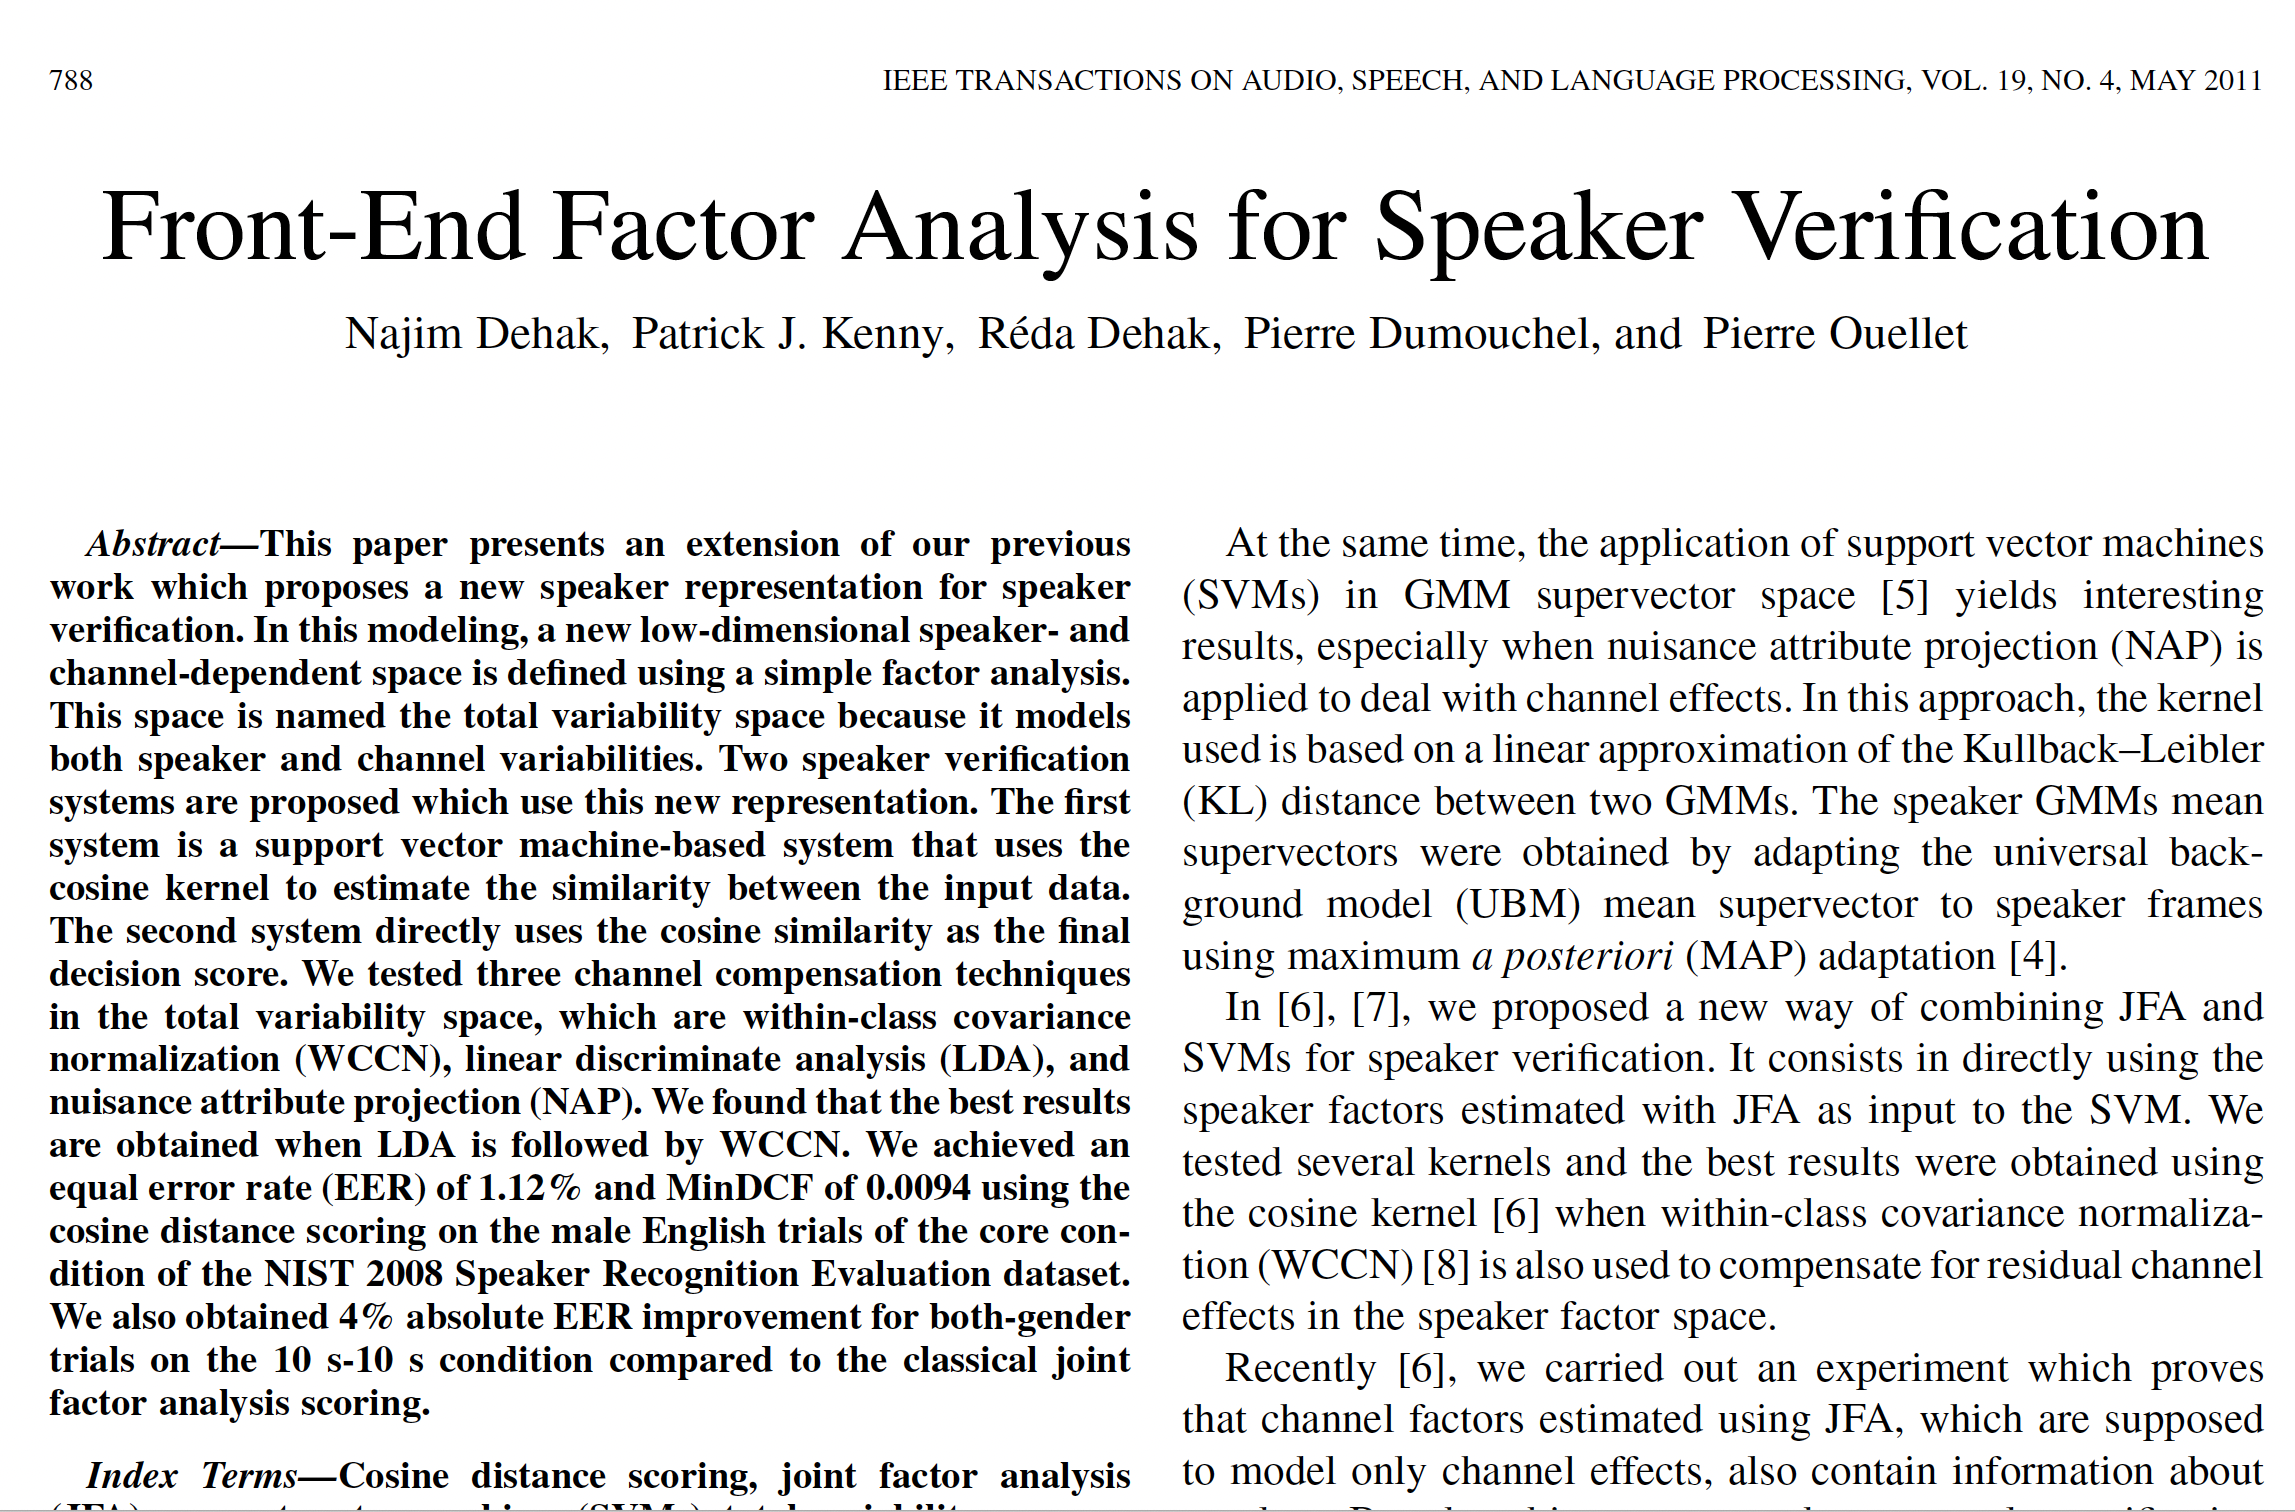
\includegraphics[width=\textwidth]{figs/dehak2011page1.png}}
\end{frame}

\begin{frame}
  \frametitle{Identity Vectors (i-vectors) Overview}

  \begin{enumerate}
  \item Convert waveform to MFCC vectors $\bm{x}_t$
  \item Gaussian mixture model soft-assigns each $\bm{x}_t$ to a phoneme.
  \item Baum-Welch computes the {\em differences} between this
    speaker's phonemes and the typical phonemes.
  \item PCA reduces the supervector to an i-vector.
  \item Measure similarity between two i-vectors using cosine similarity.
  \end{enumerate}
\end{frame}

\begin{frame}
  \frametitle{Mel Frequency Cepstral Coefficients}
  \begin{columns}
    \begin{column}{0.5\textwidth}
      \centerline{\includegraphics[width=\textwidth]{exp/melspectrogram.png}}
    \end{column}
    \begin{column}{0.5\textwidth}
      \begin{itemize}
      \item Compute STFT
      \item Convert to mel spectrogram by nonlinearly resampling the
        frequency axis, to get semi-logarithmic frequencies
      \item Convert from mel spectrogram to MFCC: approximate the PCA
        of each column using a discrete cosine transform
      \end{itemize}
    \end{column}
  \end{columns}
\end{frame}

\begin{frame}
  \frametitle{Gaussian Mixture Model}

  A Gaussian mixture model is like an HMM, but simpler:
  \begin{align*}
    \Pr\{q_t=i\} &= a_i\\
    \Pr\{\bm{x}_t|q_t=i\} &= \mathcal{N}\left(\bm{x}_t|\bm{\mu}_i,\bm{\Sigma}_i\right)
  \end{align*}

  The posterior probability of phoneme $i$ at time $t$ is therefore:
  \begin{displaymath}
    \gamma_t(i)=\Pr\{q_t=i|\bm{x}_t\}
    =\frac{\Pr\{q_t=i,\bm{x}_t\}}{\sum_k\Pr\{q_t=k,\bm{x}_t\}}
    =\frac{a_i\mathcal{N}(\bm{x}_t|\bm{\mu}_i,\bm{\Sigma}_i)}{\sum_ka_k\mathcal{N}(\bm{x}_t|\bm{\mu}_k,\bm{\Sigma}_k)}
  \end{displaymath}
\end{frame}

\begin{frame}
  \frametitle{Soft Phoneme Segmentation using GMM}

  The image below shows hard phoneme alignment.  A GMM computes soft
  phoneme alignment, $\gamma_t(i)=\Pr\{q_t=i|\bm{x}_t\}$.
  \centerline{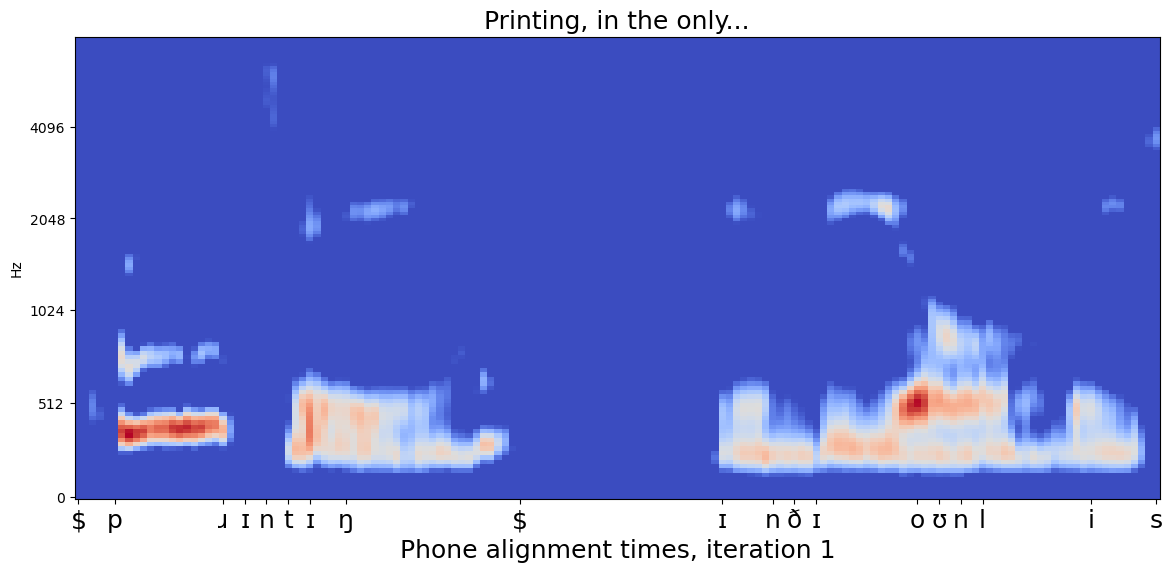
\includegraphics[width=\textwidth]{figs/segmentation.png}}
\end{frame}

\begin{frame}
  \frametitle{GMM Supervector}

  A GMM supervector lists, for each phoneme, the \textbf{differences}
  between the way in which this person produces the phoneme and the
  way in which a typical person would produce the phoneme:

  \begin{displaymath}
    \bm{s}=\left[\begin{array}{c}
        \frac{\sum_t\gamma_t(1)(\bm{x}_t-\bm{\mu}_1)}{\sum_t\gamma_t(1)}\\
        \vdots\\
        \frac{\sum_t\gamma_t(N)(\bm{x}_t-\bm{\mu}_N)}{\sum_t\gamma_t(N)}
      \end{array}\right]
  \end{displaymath}

  The dimension of this vector is very large.  Typically each
  $\bm{x}_t$ is a 40-dimensional MFCC vector, and typically there are
  2048 Gaussians, for a total $\text{len}(\bm{s})=2048\times 40=81920$.
\end{frame}

\begin{frame}
  \frametitle{i-vector}

  \begin{itemize}
  \item 
    The i-vector is a principal components analysis of the GMM supervector:
    \begin{displaymath}
      \bm{w} =\bm{G}^{-1}\bm{T}^T \bm{s}
    \end{displaymath}
    where the columns of $\bm{T}\in\Re^{81920\times 600}$ are the
    eigenvectors of the covariance of $\bm{s}$, and $\bm{G}$ is a
    diagonal normalization matrix related to the eigenvalues.
  \item
    The dimension of $\bm{w}$ is chosen to be intermediate between the
    dimension of $\bm{s}$ (81920) and the dimension of $\bm{x}_t$
    (40).  Typically, $\text{len}(\bm{w})\approx 600$.  Although
    i-vector originally meant ``identity vector,'' people sometimes
    also gloss it as ``intermediate vector.''
  \end{itemize}
\end{frame}
        
\begin{frame}
  \frametitle{Similarity}

  \begin{columns}
    \begin{column}{0.5\textwidth}
      \begin{itemize}
        \item The i-vector is a \textbf{PCA} of the
          \textbf{differences} between the test speaker's productions
          of phonemes versus the typical production.  How do we
          evaluate similarity in this space?
        \item The problem: covariances are diagonal in this space, but
          not uniform (example at right is chemical analysis, but
          speaker verification looks similar).
      \end{itemize}
    \end{column}
    \begin{column}{0.5\textwidth}
      \centerline{\includegraphics[width=\textwidth]{exp/haplogroup.png}}
      \url{https://commons.wikimedia.org/wiki/File:PCA_of_Haplogroup_J_using_37_STRs.png}
    \end{column}
  \end{columns}
\end{frame}

\begin{frame}
  \frametitle{Similarity Measures}

  The original i-vector paper tested two similarity measures:
  \begin{itemize}
  \item Directly threshold the cosine similarity:
    \begin{displaymath}
      y = \begin{cases}
        1 & \frac{\bm{w}_1^T\bm{w}_2}{\Vert\bm{w}_1\Vert\Vert\bm{w}_2\Vert}>\theta\\
        0 & \text{otherwise}
      \end{cases}
    \end{displaymath}
  \item Train a binary SVM using the cosine similarity as the kernel
  \end{itemize}
  Both of these measures, applied to i-vectors, were tested against
  joint factor analysis (JFA), the previous state of the art.
\end{frame}

\begin{frame}
  \frametitle{i-vector: Results}
  \centerline{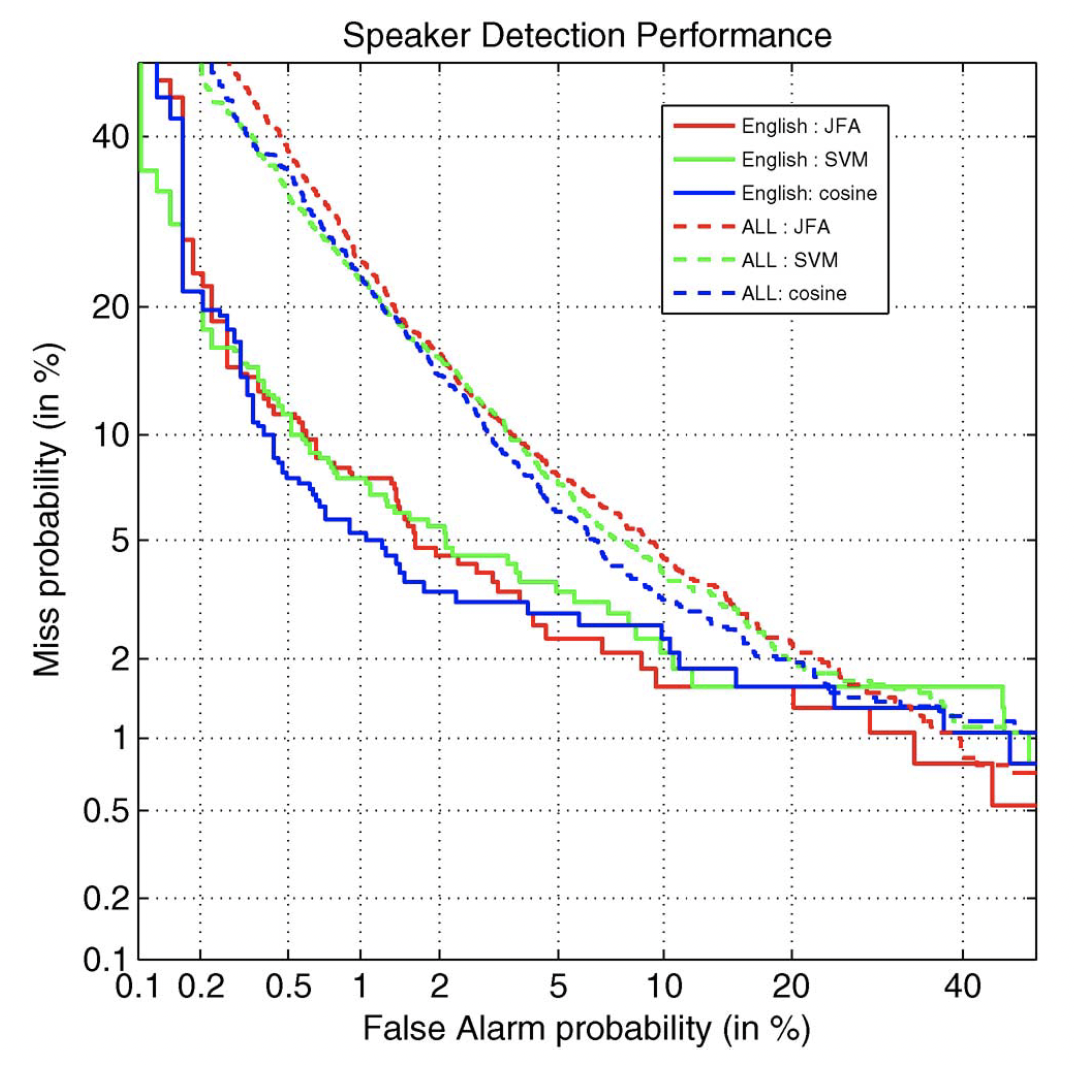
\includegraphics[height=0.8\textheight]{figs/dehak2011fig6.png}}
\end{frame}

%%%%%%%%%%%%%%%%%%%%%%%%%%%%%%%%%%%%%%%%%%%%%%%%%%%%%%%%%
\section[x-vectors]{x-vectors: Mean-Pooled CNN Supervector, PLDA Similarity}
\setcounter{subsection}{1}

\begin{frame}
  \centerline{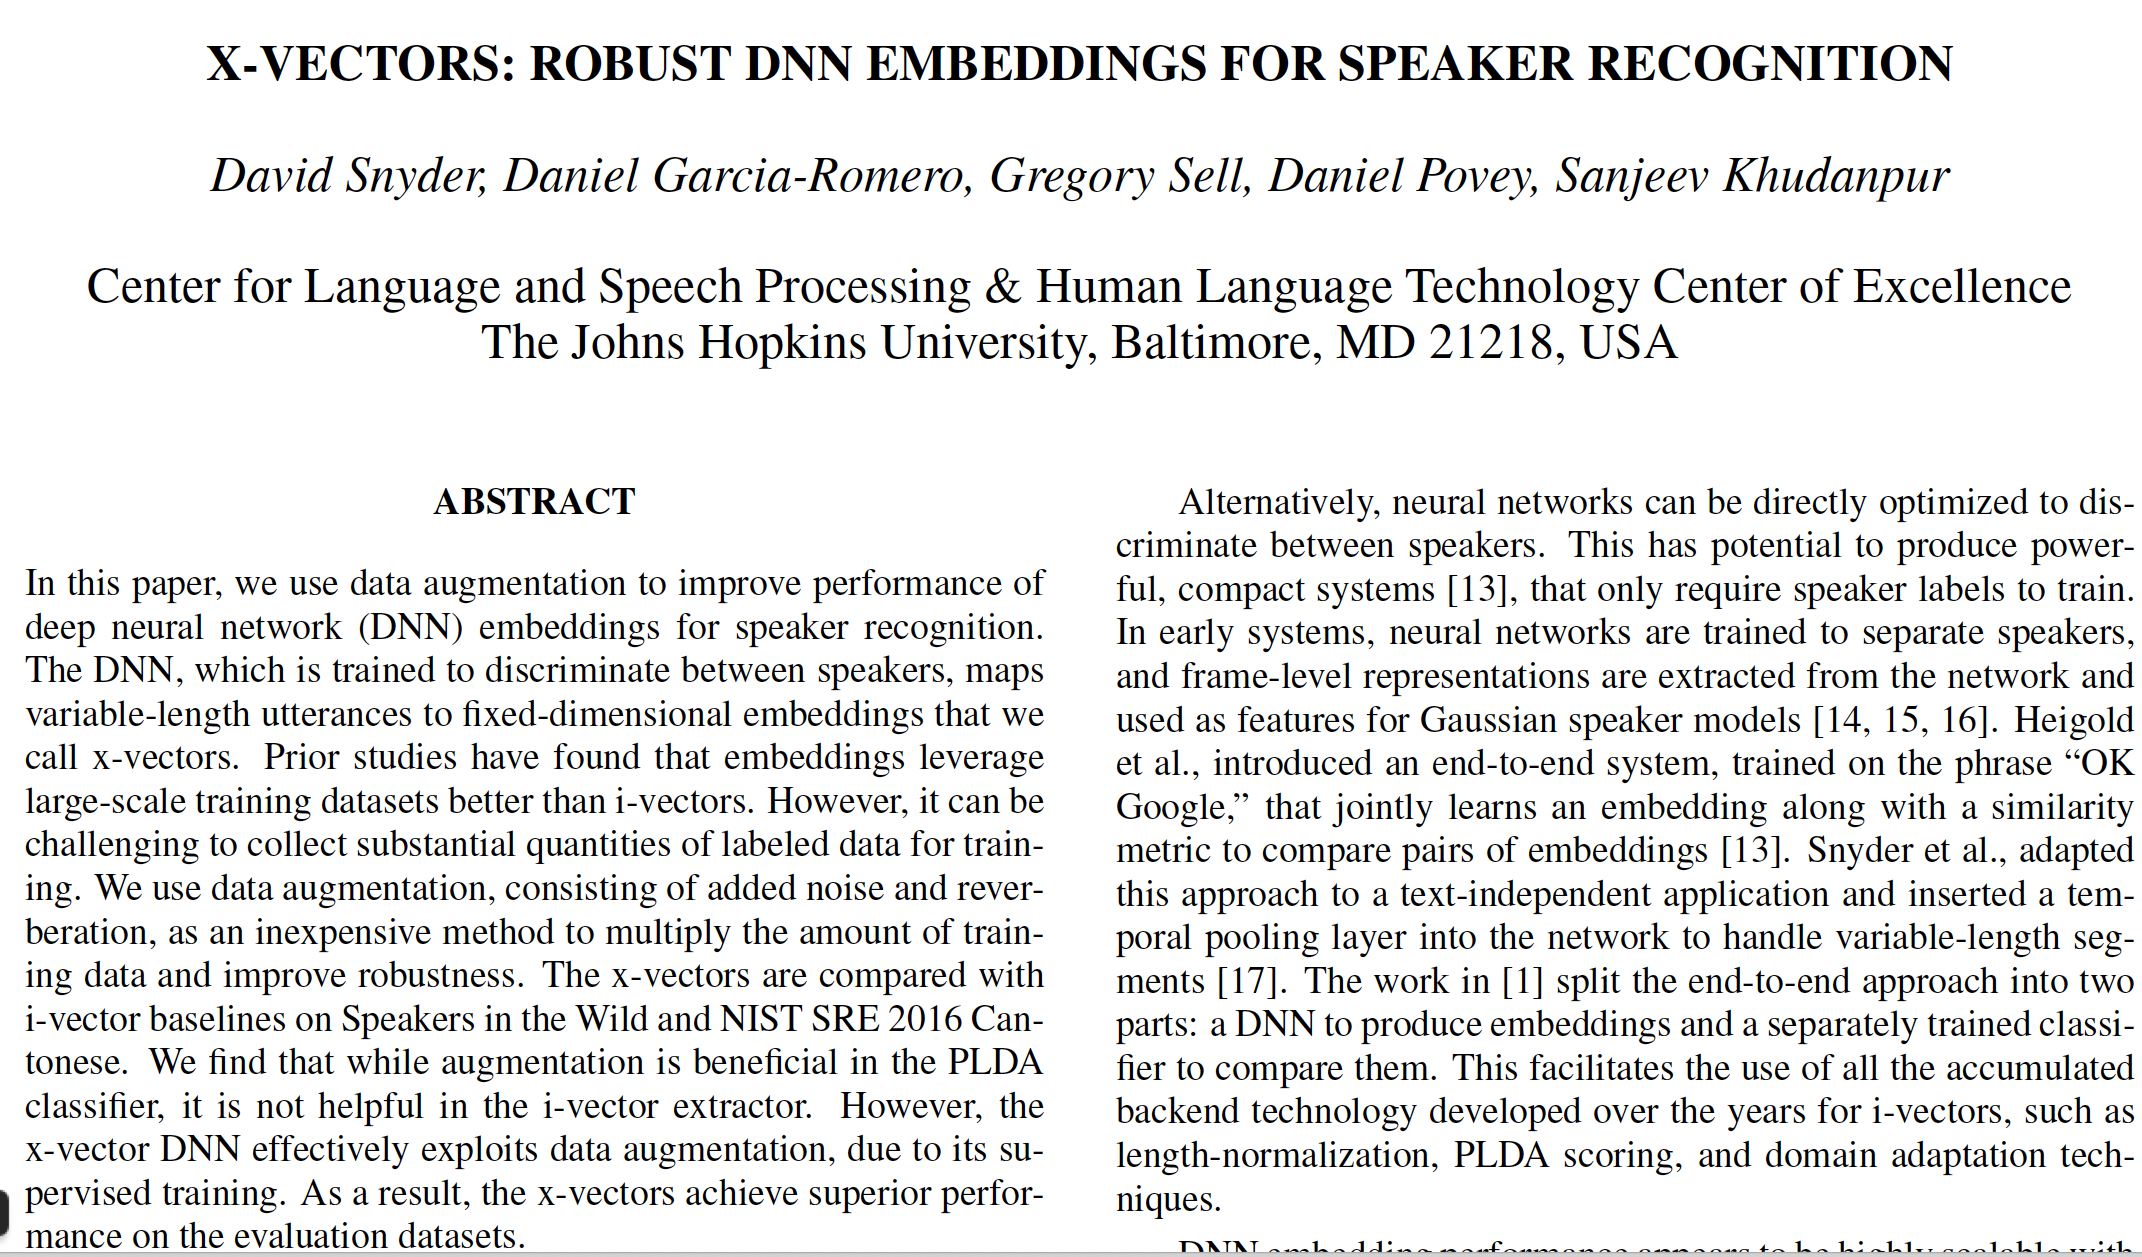
\includegraphics[width=\textwidth]{figs/snyder2018page1.png}}
\end{frame}

\begin{frame}
  \frametitle{x-vector: Acoustic features}

  Acoustic features are mel spectrograms with 40 mel bands, then
  passed through a 5-layer 1d CNN:
  \begin{displaymath}
    h^{(l)}_i[n] = g\left(\sum_{j}\sum_{m} w^{(l)}_{i,j}[m]h^{(l-1)}_j[n-m]\right)
  \end{displaymath}

  The five layers have 512, 512, 512, 512, and 1500 channels, respectively.
\end{frame}

\begin{frame}
  \frametitle{x-vector: Supervector}

  \begin{itemize}
    \item 
      The last layer of the CNN has 1500-dimensional vectors
      $\bm{h}^{(5)}[n]=[h^{(5)}_1[n],\ldots,h^{(5)}_{1500}[n]]^T$.
      That's large enough to permit different sections of the vector
      to represent mean shift of different phonemes.
    \item
      The supervector is a concatenation of the utterance mean and
      variance,
      $\bm{s}=\left[\begin{array}{c}\bm{m}\\\bm{v}\end{array}\right]$,
      where
      \begin{displaymath}
        \bm{m}=\frac{1}{N}\sum_{n=1}^N\bm{h}^{(5)}[n],~~~
        \bm{v}=\frac{1}{N-1}\sum_{n=1}^N\left(\bm{h}^{(5)}[n]-\bm{m}\right)^2
      \end{displaymath}
  \end{itemize}
\end{frame}

\begin{frame}
  \frametitle{x-vector: Intermediate vector}

  \begin{itemize}
    \item 
      The x-vector itself is a linear compression of $\bm{s}$ down to 512 dimensions:
      \begin{displaymath}
        \bm{w}=\bm{T}^T\bm{s},
      \end{displaymath}
      where $\bm{T}\in\Re^{512\times 3000}$ is a learned projection matrix.
    \item 
      The matrix $\bm{T}$ is
      trained so that a further two-layer neural net, applied to $\bm{x}$,
      classifies all of the training speakers with minimum cross-entropy.
    \item
      After training, the 2-layer network is discarded.  It's not
      needed, because none of the test speakers are in the training
      database anyway.
  \end{itemize}
\end{frame}

\begin{frame}
  \frametitle{Similarity: Probabilistic Linear Discriminant Analysis (PLDA)}

  Probabilistic linear discriminant analysis (PLDA) assumes that we a
  training set of $N$ speakers (not including the test speaker!).  The
  $i^{\text{th}}$ training speaker is represented by some x-vectors
  $\bm{w}_{i,1},\ldots,\bm{w}_{i,m}$, whose mean is
  \begin{displaymath}
    \bm{v}_i = \frac{1}{m}\sum_{j=1}^m\bm{w}_{i,j}
  \end{displaymath}
  PLDA models $\bm{v}_i$ and $\bm{w}_{i,j}$ as jointly Gaussian:
  \begin{align*}
    \bm{v}_i &\sim \mathcal{N}(\bm{v}|\bm{0},\bm{A}\bm{\Psi}\bm{A}^T)\\
    \bm{w}_{i,j} &\sim \mathcal{N}(\bm{w}|\bm{v}_i,\bm{A}\bm{A}^T),
  \end{align*}
  The matrices $\bm{A}$ and $\bm{\Psi}$ are a generalization of PCA
  called linear discriminant analysis.
\end{frame}

\begin{frame}
  \frametitle{Similarity: Probabilistic Linear Discriminant Analysis (PLDA)}

  PLDA then computes the similarity between two test vectors,
  $\bm{u}_1=\bm{A}^T\bm{w}_1$ and $\bm{u}_2=\bm{A}^T\bm{w}_2$, as

  \begin{align*}
    &R(\bm{w}_1,\bm{w}_2)=\frac{\text{likelihood}(\text{same})}{\text{likelihood}(\text{different})}\\
    &=\frac{\int\Pr(\bm{u}_1,\bm{u}_2,\bm{v})d\bm{v}}{\left(\int\Pr(\bm{u}_1,\bm{v}_1)d\bm{v}_1\right)\left(\int\Pr(\bm{u}_2,\bm{v}_2)d\bm{v}_2\right)}
  \end{align*}
  If we set $\bar{\bm{u}}=\frac{1}{2}\left(\bm{u}_1+\bm{u}_2\right)$, then we can write:
  \begin{align*}
    R(\bm{w}_1,\bm{w}_2)
    &\propto\frac{\mathcal{N}\left(\bar{\bm{u}}\vert\bm{0},\bm{\Psi}+\frac{1}{2}\bm{I}\right)\mathcal{N}\left(\bm{u}_1\vert\bar{\bm{u}},\bm{I}\right)\mathcal{N}\left(\bm{u}_2\vert\bar{\bm{u}},\bm{I}\right)}{\mathcal{N}\left(\bm{u}_1\vert\bm{\Psi}+\bm{I}\right)\mathcal{N}\left(\bm{u}_2\vert\bm{\Psi}+\bm{I}\right)},
  \end{align*}
\end{frame}



\begin{frame}
  \frametitle{Similarity: Probabilistic Linear Discriminant Analysis (PLDA)}

  Two test utterances are then judged to have come from the same
  speaker if their PLDA score is above a threshold:
  \begin{displaymath}
    y =\begin{cases}
    1 & R(\bm{w}_1,\bm{w}_2)>\theta\\
    0 &\mbox{otherwise}
    \end{cases}
  \end{displaymath}
\end{frame}

\begin{frame}
  \frametitle{x-vector: Results}

  \centerline{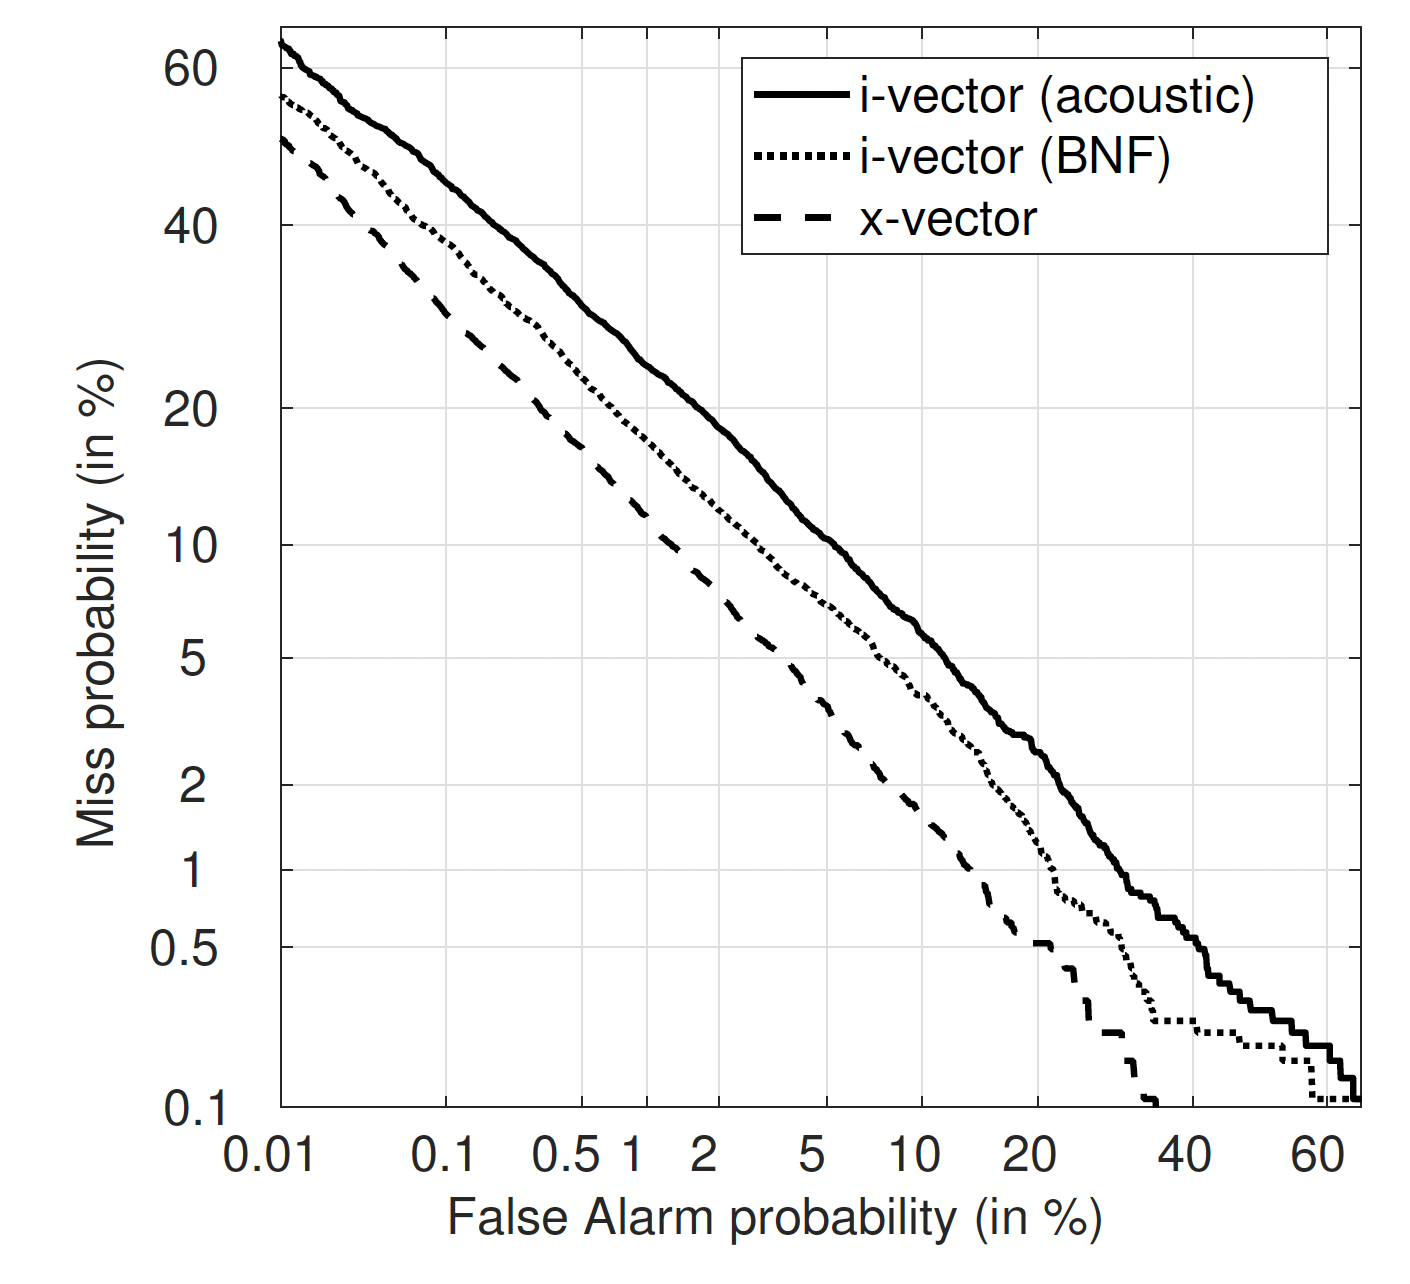
\includegraphics[height=0.8\textheight]{figs/snyder2018fig2.png}}
\end{frame}

%%%%%%%%%%%%%%%%%%%%%%%%%%%%%%%%%%%%%%%%%%%%%%%%%%%%%%%%%
\section[d-vectors]{d-vectors: LSTM Supervector, Cosine Similarity}
\setcounter{subsection}{1}

\begin{frame}
  \centerline{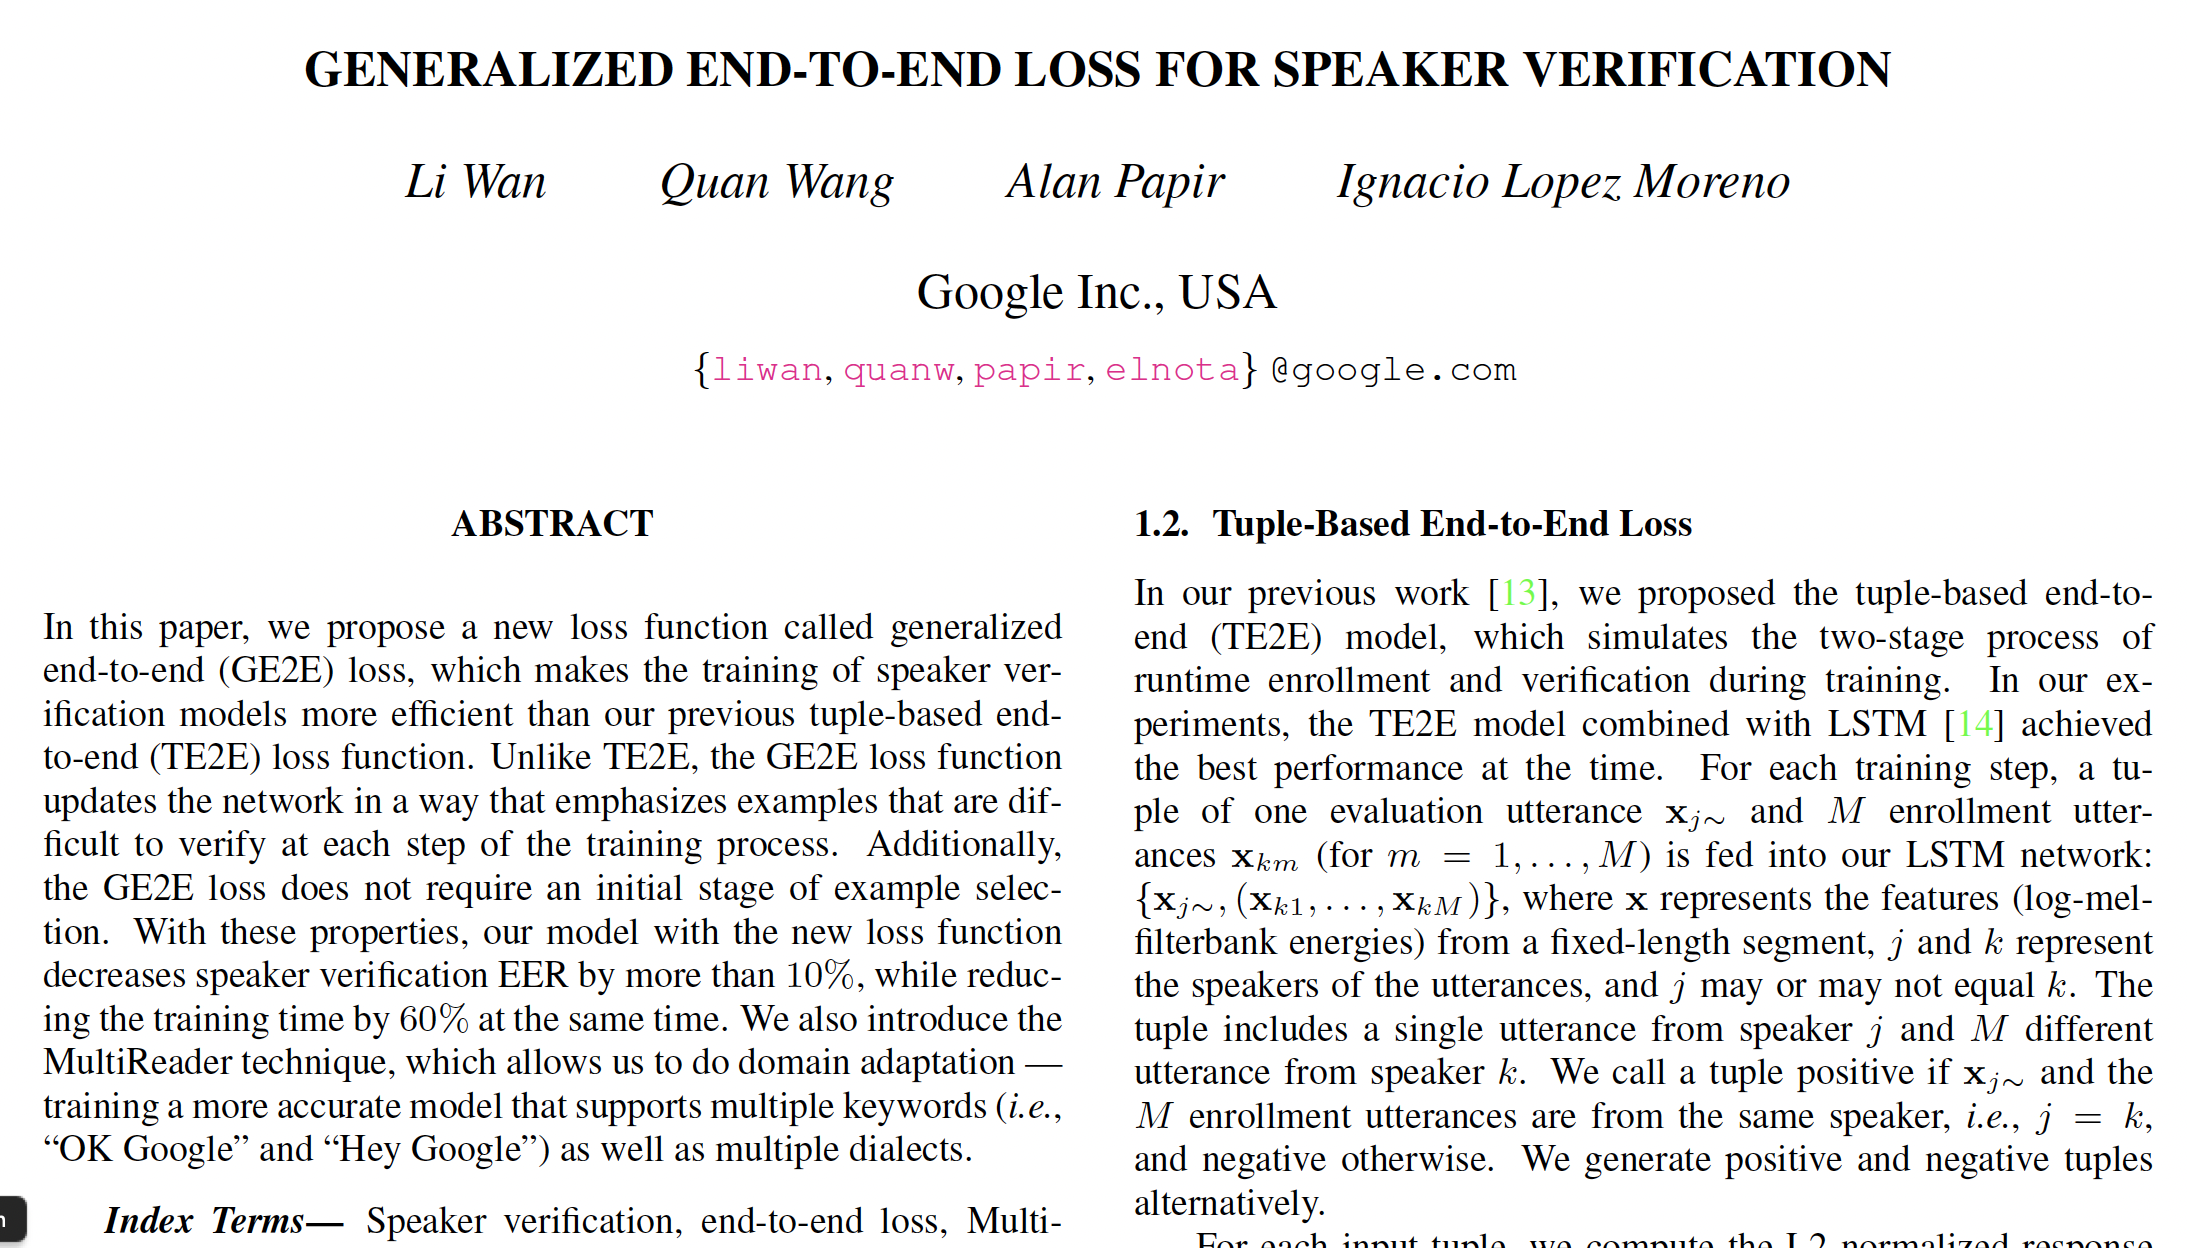
\includegraphics[width=\textwidth]{figs/wan2018page1.png}}
\end{frame}

\begin{frame}
  \frametitle{d-vector: Overview}

  \begin{itemize}
  \item Acoustic features: 40 Mel filterbank coefficients
  \item Supervector = 768d state vector of a unidirectional LSTM after the end of the utterance
  \item Intermediate vector (d-vector) = 256d linear projection of the supervector
  \item Similarity score: cosine similarity
    \begin{displaymath}
      y=\begin{cases}
      1 & \frac{\bm{w}_1^T\bm{w}_2}{\Vert\bm{w}_1\Vert\Vert\bm{w}_2\Vert} >\theta\\
      0 &\mbox{otherwise}
      \end{cases}
    \end{displaymath}
  \end{itemize}
\end{frame}

\begin{frame}
  \frametitle{Supervector = 768d state vector of a unidirectional LSTM}

  Run the following system over a length-$T$ entire utterance:

  \centerline{\includegraphics[height=0.5\textheight]{exp/lstm.png}}
  \centerline{\footnotesize{\url{https://commons.wikimedia.org/wiki/File:Long_Short-Term_Memory.svg}}}

  \vspace*{1mm}
  
  \ldots then $\bm{h}_T$ is the supervector, and $\bm{o}_T$ is the 256d d-vector.
\end{frame}

\begin{frame}
  \frametitle{End-to-end training}

  Test speakers are not in the training set!  Nevertheless, end-to-end
  training is possible if your training set has a large enough number
  of speakers.  In that case you can use:
  \begin{align*}
    \mathcal{L} &= \sum_{j=1}^{\text{\# speakers}}\sum_{i=1}^{\text{\# utterances}}
    \log\left(\frac{e^{\cos(\bm{w}_{j,i},\bar{\bm{w}}_j)}}{\sum_{k=1}^{\text{\# speakers}} e^{\cos(\bm{w}_{j,i},\bar{\bm{w}}_k)}}\right)\\
    \cos(\bm{w}_{j,i},\bar{\bm{w}}_k) &= \frac{\bm{w}_{j,i}^T\bar{\bm{w}}_k}{\Vert\bm{w}_{j,i}\Vert\Vert\bar{\bm{w}}_k\Vert},
  \end{align*}
  where $\bar{\bm{w}}_k$ is the average d-vector computed from utterances of speaker $k$.
\end{frame}


\begin{frame}
  \frametitle{End-to-end training}

  Test speakers are not in the training set!  Nevertheless, end-to-end
  training is possible if your training set has a large enough number
  of speakers:
  \begin{itemize}
  \item i-vector was trained using 1,748 speakers
  \item x-vector was trained using 2,600 speakers, but only beat
    i-vector if it used data augmentation during training
  \item d-vector was trained using 648,000 speakers
  \end{itemize}
\end{frame}

\begin{frame}
  \frametitle{d-vector: Results}
  
  \centerline{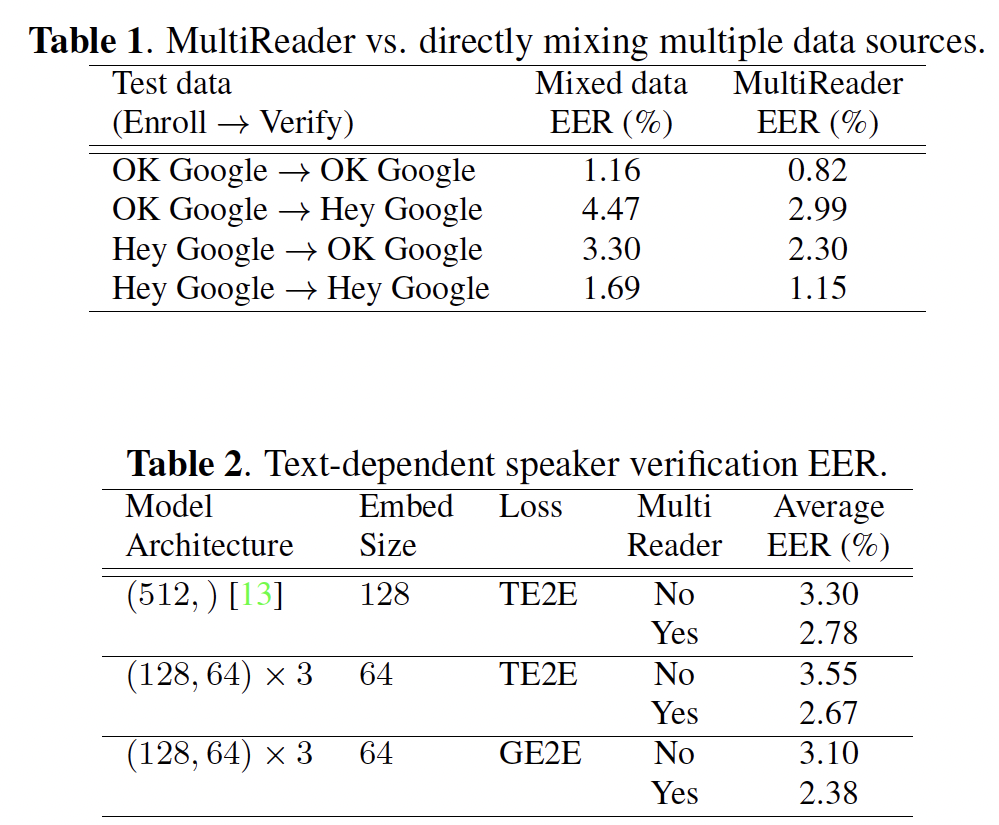
\includegraphics[height=0.8\textheight]{figs/wan2018table1.png}}
\end{frame}

  
%%%%%%%%%%%%%%%%%%%%%%%%%%%%%%%%%%%%%%%%%%%%%%%%%%%%%%%%%
\section{Summary}
\setcounter{subsection}{1}


\begin{frame}
  \frametitle{Comparison of Systems}

  \begin{center}
    \begin{tabular}{|p{15mm}|p{30mm}|p{16mm}|p{13mm}|p{13mm}|}\hline
      System & Supervector & Projection & Similarity & Training Speakers\\\hline
      i-vector & Mean shift of GMM centroids & PCA & cos & 1,748\\
      x-vector & Mean and variance of 1500d CNN output & learned & PLDA & 2,600\\
      d-vector & Last state of LSTM & learned & cos & 648,000\\\hline
    \end{tabular}
  \end{center}
\end{frame}

\end{document}

